% EPC flow charts
% Author: Fabian Schuh
\documentclass{article}
\usepackage{myflowchart}

\begin{document}

\begin{tikzpicture}

\begin{scope}[node distance=5mm and 5mm]

\node [ item=4](a) at (1,1) {%
            \textbf{擴充}
            \nodepart{two}
            \begin{enumerate}
            	\item gyro sensor轉動驗證,準確性歸納。應用?
            	\item Chatter ring, fidget spinner模擬驗證。
		\item 兵乓球碰撞後旋轉模擬。
            	\item 結合疊格來做立體作圖?
            	\item 增加藍芽傳輸(沒有wifi時)
            	\item 與ejss準確度比較
            	\item 偏移誤差近似與改進(與ejss,sensor轉動驗證均有關係)
            	\item 加光線追蹤美觀化?換白色cube?
            	\item unity3D飛機滑鼠控制器?
           \end{enumerate}
           \nodepart{three}\textbf{待修正事項}
	\nodepart{four}
	\begin{enumerate}
            \item GUI設計卡住,見第二頁討論
            \item OpenGL animation關閉後要手動重啟一個新個interpreter,因為glut的關係,怎麼改進?
            \item py2exe作業系統可執行檔,軟體化
            \item mplot3D例子全換OpenGL?
            \item OpenGL動畫延遲,不能漏接貼角。
            \item 製作gimbal中...
	\end{enumerate}
            };

\node [gitrec,below=of a](b)   
{git log}edge [<-,>=stealth'] (a);

\node [item=2,below=of b](c)
{%
\textbf{模擬軟體擴充}
\nodepart{two}
\begin{enumerate}
            \item 增加新模擬,包括物理引擎python與OpenGL動畫呈現。動畫物體的繪製也很花時間。
            \item 寫程式函式說明,update演進紀錄changelog,(comment \& documentation \& update log)
            \item 用py2exe調整做成exe
\end{enumerate}
}edge [<-,>=stealth'] (b);

\node [gitrec,below=of c](d)   
{git log}edge [<-,>=stealth'] (c);

\node [item=2,below=of d](e)
{%
\textbf{pdf文件}
\nodepart{two}
\begin{enumerate}
            \item 製作要放入文件的圖片(疊格技術運用)
            \item 以Scientific Word軟體撰寫擴充的新內容,寫軟體操作說明,然後使用本工作室開發的自動化流程來進行章節或全書的編譯(使用Xelatex引擎),來產生PDF技術文件。
            \item 列印,技術文件裝訂成冊
\end{enumerate}
}edge [<-,>=stealth'] (d);

%draw the curve line
%\draw [->,out = 180, in = 0] (h) to  (f);



\node [phantom, below right=of a.north east](gic2){};
\node [phantom, right=of e](gic1){};

\node [item=2,below right = of gic2](g)
{\textbf{加入網頁}
\nodepart{two}
\begin{enumerate}
            \item 製作網頁可觀看的示範影片
            \item Landing page的修改。以LYX增加Landing page的新內容,然後利用LYX的HTML export功能,若有數學要加上使用Mathjax的選項。然後git push上pyanywere網站。
            \item 有時也需要把技術文件po上網頁,做成blog文章,此時就利用SW中的export HTML功能。需要時要微調。例如production chapter。
\end{enumerate}
};%edge [<-,>=stealth'] (f);

\node [gitrec,above=of g](f)   
{git log}edge [->,>=stealth'] (g);

\node [above right = of a.north east, align=center, anchor = south] (title){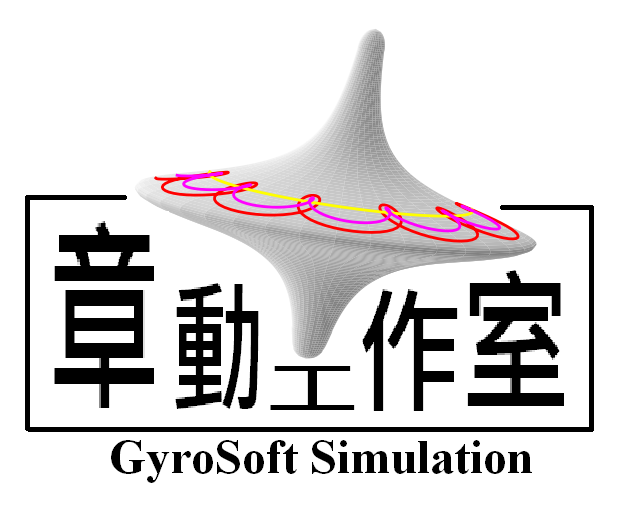
\includegraphics[width=0.4\textwidth]{../../figs/test_new_logo_chinese.png}\\ \LARGE 作業流程};

\draw [rounded corners,->,>=stealth'] (e) --  (gic1.center) -- (gic2.center) -- (f);


\node [item=2,below=of g](h)
{%
\textbf{推廣(找專人負責)}
\nodepart{two}
\begin{enumerate}
            \item 陀螺儀應用體驗店
            \item 廣告文宣製作,以landing page製作flyer。將LYX中landing page的內容export成xetex碼,然後在texlive按照我們整理好的方式修改成Texlive的xelatex可編譯碼,然後編譯成PDF flyer。列印後發放。
            \item gss logo不同型式的製作,名片電繡等製作。
\end{enumerate}
}edge [<-,>=stealth'] (g);


\end{scope}
\end{tikzpicture}

% second page
\begin{tikzpicture}[item]
\begin{scope}[node distance=5mm and 5mm]

\node [ item=2](thinking) at (1,1) {%
            \textbf{思考}
            \nodepart[text width = 8.2cm]{two}
            \begin{enumerate}
            	\item GUI使用者自訂參數程式有進展但未完成,GUI module加說明
            	\begin{enumerate}
            		\item 想把GUI弄成方便驗證self-energized fidget spinner,但這樣的話需要能夠以GUI方式給力矩,不太可能歐...這裡連問題都不知道是甚麼,不需要做GUI,等到知道問題後再為了方便性做GUI才較好。
            		\item GUI的目的是將目前所有功能統整呈現,方便操作方便探索,所以應是針對現有已完成的例子。
			\item 所以應該是先將gyro demo做成可輕易更改參數,然後可方便觀看AB法的差異。
			\item 然後C法應該是姿態估測的,或許應該跟gyro demo做切割?所以ABC三法應該要切割一下?
		\end{enumerate}
		\item 階段任務算告一段落。事實上py檔都可獨立跑,GUI實在有點太難,不做了,放下。
		\item 將目前東西完整記錄,整理,建檔就已經很花時間,做不完了。
            \end{enumerate}
            };

\node [above right = of thinking, align=center, anchor = south] (title){\parbox[c][][c]{0.3\textwidth}{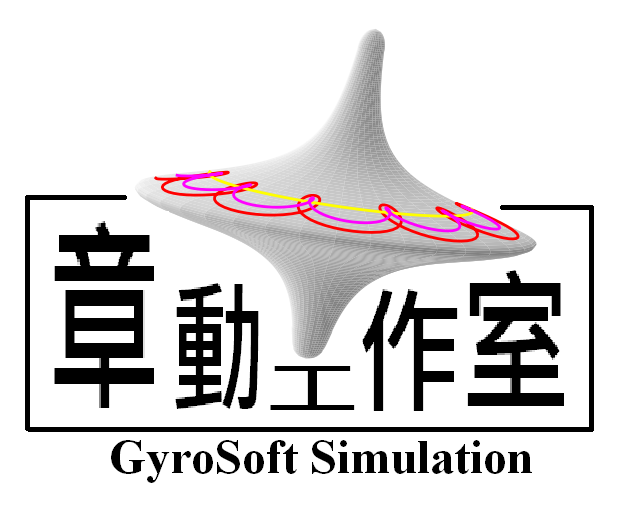
\includegraphics[width=0.3\textwidth]{../../figs/test_new_logo_chinese.png}}\parbox[c][][c]{7cm}{\Huge 卡住kazoo}};

\end{scope}
\end{tikzpicture}
% end second page
\end{document}
